\documentclass{report}
\usepackage{fullpage}
\usepackage[margin=0.5in]{geometry}
\usepackage{hyperref}
\usepackage{amsfonts}
\usepackage{float}
\usepackage{graphicx}
\usepackage{caption}
\usepackage{subcaption}
\renewcommand{\baselinestretch}{2}
\author{Steven Englehardt, Maciej Halber, Elena Sizikova}
\title{Understanding Collections of Images \\ \small{COS 521 Final Project Report}}
\begin{document}
\maketitle
\tableofcontents

\chapter{Introduction}
\section{Abstract}
This report explores a variety of image properties that make it possible to understand vast collections of images. In particular, we look at how image color, saturation, sharpness, and detail can be extracted and compared between images using methods such as Fast Fourier Transform (FFT) and Singular Value Decomposition (SVD). We seek to understand how the theoretical underpinnings of these two algorithms affect the way the images are created in the first place. Ultimately, we provide a way of decomposing the image into mathematical notation (a descriptor) that differentiates well between a collection of images.

\section{Background Work}
There are many possible situations in which we would need to understand and compare image structure. For example, one might like to search for a location in which a photograph was taken, by looking at all the other available images, and finding the image closest to the search image. Alternatively, one may want to cluster images based on their content, and see what categories the image collection can be decomposed to. Both of these would be easy problems to solve, if the images were annotated with words: textual search is a well-solved problem. However, when the images are not labelled (this is known as unsupervised learning), and the image collection is extremely large, it is impractical to label the images by hand. For such problems, it is important to analyze image content automatically.

Existing methods of image search by analyzing content of the image include Google Goggles and Google Image Search, both are based on similar technology \cite{google_blog}, which checks for distinctive points, analyzes lines and textures and finally creates a mathematical model of the image. While the exact implementation is not available, Google Image Search does not provide clustering capabilities of analyzing existing input datasets. A more closer work is that of Oliva and Torralba \cite{gist_descriptor} which create a GIST descriptor (cite Freedmans work!!!), and use perceptual dimensions (naturalness, openness, roughness, expansion, ruggedness) to classify natural images, for example, pictures of coasts, mountains or cities. The authors work with a low dimensional representation of the scene which is collectively known as the \emph{Spatial Envelope}. The properties of the spatial envelope are estimated by means of Discrete Fourier Transform (DFT), Windowed Fourier transform (WFT), as well as spectral properties of the image are estimates (!!!! Expand). 

Having completed a graduate course in algorithms, our goal was to understand the results that were obtained by such a study, and specifically answer the question: why can we estimate proporties of the spatial envelope the way \cite{gist_descriptor} does? 


\chapter{Methods}
Three directions of image analysis were analyzed and tested. We first started with a collection of color images that were analyzed by the method of Color Histograms. We also analyzed the properties of the FFT method and the SVD method on the corresponding greyscale images. The resulting descriptors were then compared against each other and subsequently combined into a joint descriptor, that used the information from all three methods to describe images.

\section{Data}
We tested the descriptors on two data-sets ?????
\section{Implementation}

When factoring images using SVD or working with the FFT of an image, we chose to work in grayscale. The choice to do so was motivated by the desire to explore the physical meaning of the decomposition or transformation in the context of images. Though it is entirely possible to separate the red, green, and blue channels and work with each separately, it is difficult to determine whether relative differences in colors or deeper properties of the decomposition/transformation are leading to the observed descriptor performance. To do the conversion we used matlab's built-in \textit{rgb2gray} function, which removes hue and saturation information but preserves luminance. [[I originally was going to discuss this in the SVD section, but I think it fits well here.]]

\section{Color Analysis}
We began the exporation of image properties by considering the color analysis method. In particular, the range of image colors that can be seen on a computer monitor are known as \emph{gamut}, see \cite{color_model_ref}. As we only considered computer images in .jpg and .png formats, we were mainly concerned with the models that represent the gamut. One of the most common such models is known as the RGB model, in which color at every pixel is a combination of three intensity values, of the Red, Green, and Blue colors.  
\begin{figure}[hbtp]
\centering
\caption{RGB Cube Model}
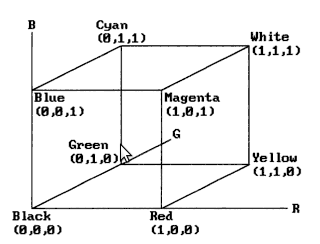
\includegraphics[scale=0.5]{graphics/rgb_cube.png}
\end{figure}






\section{Fast Fourier Transform (FFT)} (????? what is the 2D FFT in terms of FFT)
A $2$-dimensional FFT of a (grayscale) image is a transformation from the spatial domain to the frequency domain. In the spatial domain, an image is represented by function $f(x,y)$ on all relevant points $(x,y)$ in  $\mathbb{R}^2$. In the frequncy domain, the image is represented by a function $F(u,v)$ where $u$ and $v$ are frequency values. It follows that in the frequency decomposition, an image is represented by a matrix of complex values $F$, where $F(u,v)$ encodes the amplitude and the phase of the frequencies $u$ and $v$. Mathematically, the $2$-D FFT is defined as:
\begin{eqnarray}
F(u,v) = \int \int ^{\infty}_{-\infty} f(x,y)e^{-j2\pi (ux+vy)}dx dy
\end{eqnarray}
For $n$ points, we can compute the $1$-D DFT efficiently in $O(n\log{n})$ operations. The Matlab implemetation of the $2$-D FFT is extremely  fast, and we had no computational time issues with basing descriptors on these computations.

\subsection{Localization}
To understand the properties of the $2$-D FFT, we started by analyzying the $1$-D FFT first. Consider the following functions, and their representations in the Fourier domain (\ref{fig:fft_localization}). A plot of $f(x)=\cos {x}$ is not localized in the spatial domain, but is localized in the Fourier domain: it is represented by a single peak. Conversely, $g(x)=\cos {50x}$ is localized in the spatial domain, as it consists of oscillations around $x=0$. In the Fourier domain, the same function is no longer localized. This example is representative of the behavior of FFT, and suggested us a  way of how to tackle images in the Fourier domain.
\begin{figure}[h]
        \centering
        \begin{subfigure}[b]{0.2\textwidth}
                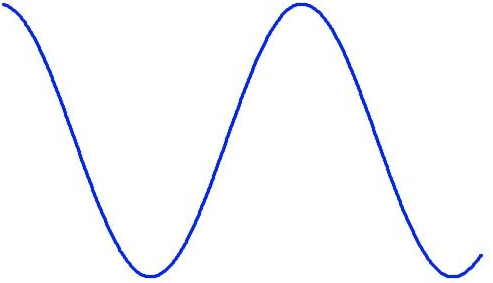
\includegraphics[width=\textwidth]{graphics/graph_fft_1.jpg}
                \caption{$f(x)=\cos{x}$}
                \label{fig:gull}
        \end{subfigure}%
        ~
         %add desired spacing between images, e. g. ~, \quad, \qquad etc.
          %(or a blank line to force the subfigure onto a new line)
        \begin{subfigure}[b]{0.2\textwidth}
                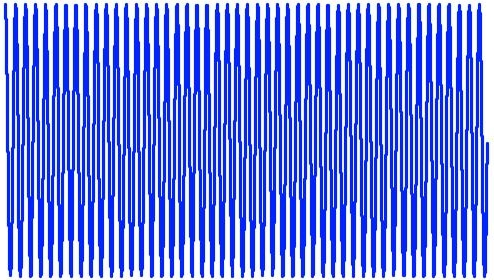
\includegraphics[width=\textwidth]{graphics/graph_fft_2.jpg}
                \caption{$g(x)=\cos{50x}$}
                \label{fig:tiger}
        \end{subfigure}
        
         %add desired spacing between images, e. g. ~, \quad, \qquad etc.
          %(or a blank line to force the subfigure onto a new line)
        \begin{subfigure}[b]{0.2\textwidth}
                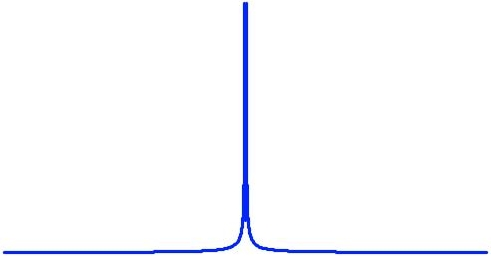
\includegraphics[width=\textwidth]{graphics/graph_fft_3.jpg}
                \caption{$F(f(x))$}
                \label{fig:mouse}
        \end{subfigure}
        ~
        \begin{subfigure}[b]{0.2\textwidth}
                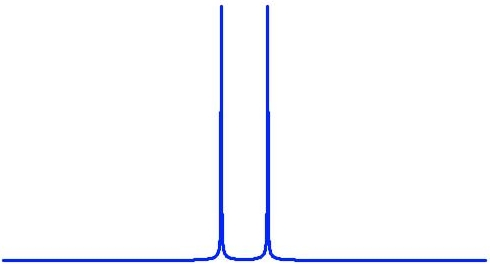
\includegraphics[width=\textwidth]{graphics/graph_fft_4.jpg}
                \caption{$F(g(x))$}
                \label{fig:mouse}
        \end{subfigure}
        \caption{Example of localization properties of different functions in the spatial and Fourier domains. Images localized in the spatial domain are not localized in the Fourier domain, and vice versa.}\label{fig:fft_localization}
\end{figure}

The given analysis yielded an easy descriptor, in which we sorted the images according the increasing contribution of low frequencies (alternatively, the decreasing contribution of high frequencies) \ref{fig:fft_low_freq_order} (!!!!!! Maciej, how exactly did you generate this?? Is this based on amplitude?). The images should be read as one line that wraps from right to left. 
\begin{figure}[hbtp]
\centering
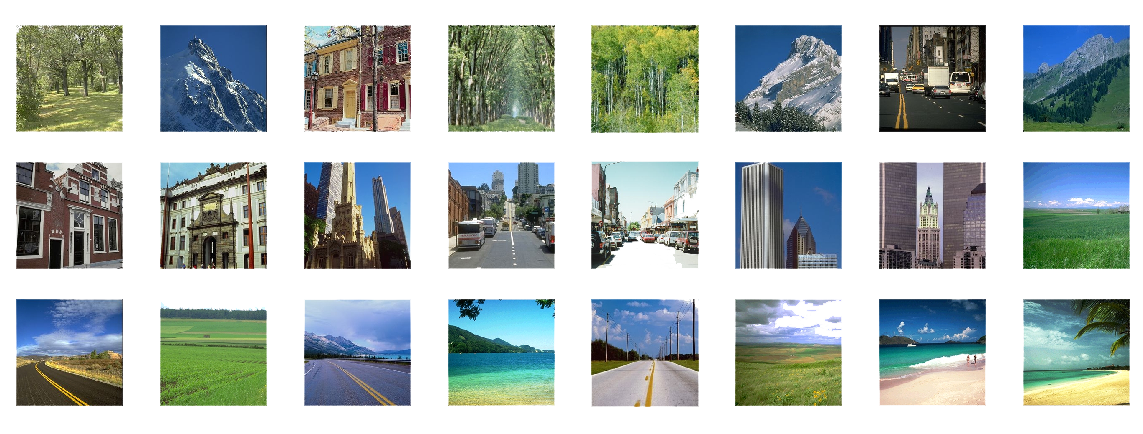
\includegraphics[scale=0.3]{graphics/FrequencyOrdered.png}
\caption{Ordering of a Subset of the ???? Dataset by Increasing Contribution of Low Frequencies}
\label{fig:fft_low_freq_order}
\end{figure}
One can see that the images on the left side of the spectrum, with a lot of contribution from high frequencies and not so much from low frequencies have many small details: they show leaves, rock incisions on the mountain, and fine building facade. In comparison, the images at the right side of the spectrum are images of open country, roads, and beaches. These images are simple, in the sense that they have a dominant horizon line and not so much small detail. It follows that these images are described mostly by low frequencies, and not by high frequencies. Notice that this analysis discards a lot of information about the distribution of frequency contribution. We therefore proceeded into analyzing both phase and amplitude footprints of the image in greater detail.



\subsection{Amplitude and Phase Analysis}
Consider the decomposition of an image of a building in a city from the (???????????) GIST dataset into its frequency and amplitude footprints.
\begin{figure}[H]
        \centering
        \begin{subfigure}[b]{0.2\textwidth}
                
\includegraphics[width=\textwidth]{graphics/original.png}
                \caption{Original image}
                \label{fig:gull}
        \end{subfigure}%
        ~
         %add desired spacing between images, e. g. ~, \quad, \qquad etc.
          %(or a blank line to force the subfigure onto a new line)
        \begin{subfigure}[b]{0.2\textwidth}
                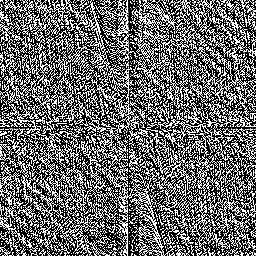
\includegraphics[width=\textwidth]{graphics/phase.png}
                \caption{Phase}
                \label{fig:mouse}
        \end{subfigure}
        ~
         %add desired spacing between images, e. g. ~, \quad, \qquad etc.
          %(or a blank line to force the subfigure onto a new line)
        \begin{subfigure}[b]{0.2\textwidth}
                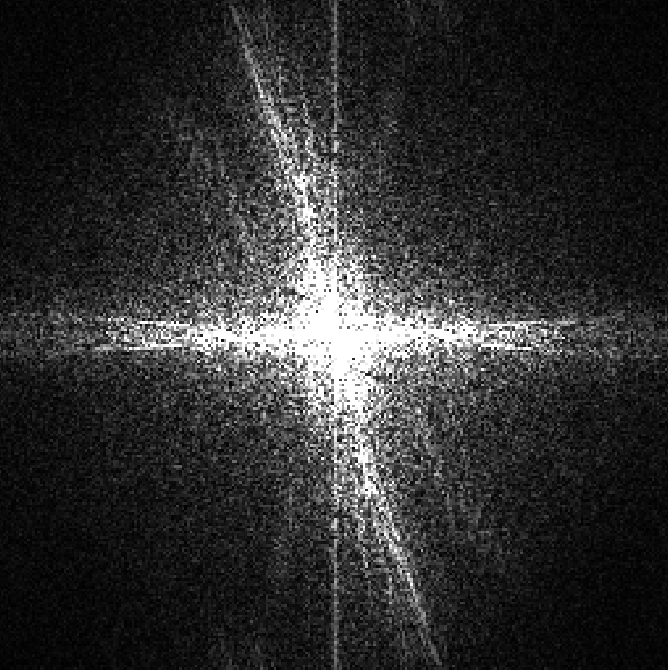
\includegraphics[width=\textwidth]{graphics/ampl.png}
                \caption{Amplitude}
                \label{fig:tiger}
        \end{subfigure}
        ~
        \begin{subfigure}[b]{0.2\textwidth}
                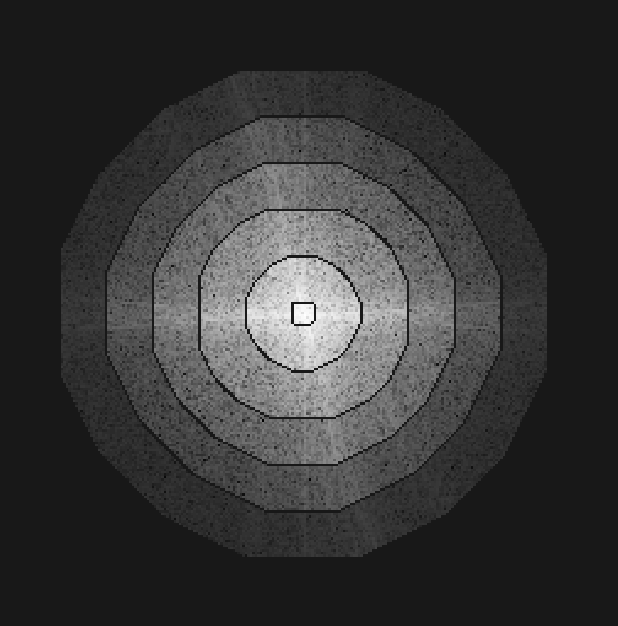
\includegraphics[width=\textwidth]{graphics/freq_bins.png}
                \caption{Frequency Bins}
                \label{fig:mouse}
        \end{subfigure}
        \caption{Example of localization properties of different functions in the spatial and Fourier domains. Images localized in the spatial domain are not localized in the Fourier domain, and vice versa.}\label{fig:fft_localization}
\end{figure}
As Oliva writes in \cite{gist_descriptor}, the phase image represents local properties of the image. It contains information relative to the form and the position of image components, while the amplitude talks about orientation, smoothness,
length and width of the contours in the given image. This can be further understood by taking the true phase values of the image, and setting all the amplitude values to $1$ (effectively taking out all amplitude variation and flattening the image), or taking true amplitude values and randomizing the phase:
\begin{figure}[H]
        \centering
        \begin{subfigure}[b]{0.2\textwidth}
                
\includegraphics[width=\textwidth]{graphics/original.png}
                \caption{Original image}
                \label{fig:gull}
        \end{subfigure}%
        ~
         %add desired spacing between images, e. g. ~, \quad, \qquad etc.
          %(or a blank line to force the subfigure onto a new line)
        \begin{subfigure}[b]{0.2\textwidth}
                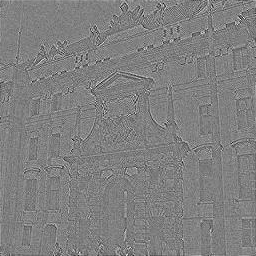
\includegraphics[width=\textwidth]{graphics/flat_power.jpg}
                \caption{Flat amplitude}
                \label{fig:mouse}
        \end{subfigure}
        ~
         %add desired spacing between images, e. g. ~, \quad, \qquad etc.
          %(or a blank line to force the subfigure onto a new line)
        \begin{subfigure}[b]{0.2\textwidth}
                
\includegraphics[width=\textwidth]{graphics/randomized_phase.jpg}
                \caption{Randomized phase}
                \label{fig:tiger}
        \end{subfigure}
        \caption{Analysis of Contributions of both Phase and Amplitude to an Image}\label{fig:fft_randomization}
\end{figure}
Note that a reconstructed image in which the amplitude information was not preserved retains the information about the edges and outlines in the original image. Conversely, the amplitude-preserved image is meaningless to out eyes: it shows the distribution and concentration of color. 




\section{Singular Value Decomposition}
A deeper understanding of Singular value decomposition (SVD) in the context of images allows the creation of a descriptor that captures overall image complexity in a relatively small descriptor length. SVD is a factorization of any real or complex 2-dimensional matrix. Since images will always be represented by real matrices, we ignore the complex case in our analysis. An $m \times n$ matrix $A$ has an SVD defined by:
$$A_{\scriptscriptstyle m \times n} = U_{\scriptscriptstyle m \times m}S_{\scriptscriptstyle m \times n}V_{\scriptscriptstyle n \times n}^T$$
where $S$ is a diagonal $m \times n$ matrix with the singular values of $A$ on the main diagonal (in decreasing order). The columns of $U$ and $V$ are known as the left and right singular vectors of $A$, respectively. $U$ and $V$ are orthonormal matrices, and the columns are basis vectors for the reconstruction. It is useful to think of each singular value in $S$ as scaling the basis vectors from $U$ and $V$ to generate an 'eigenimage' \cite{svd_image_coding}, or the contribution of that specific singular value to the overall image.

[[ Perhaps it makes sense to go a bit more in depth here on the mathematical definition of singular values given on \url{https://en.wikipedia.org/wiki/Singular_value} and \url{https://en.wikipedia.org/wiki/Singular_value_decomposition#Singular_values.2C_singular_vectors.2C_and_their_relation_to_the_SVD}
]]

With this perspective, we 

\chapter{Analysis}

\chapter{Suggestions for Further Work}
%\subsection{Your Subsection title here}
%\subsubsection{Your subsubsection title here}
%\paragraph{Your paragraph title here}


\begin{thebibliography}{9}

\bibitem{google_blog}
  Johanna Wright,
  \emph{Search by Text, Voice, or Image}.
  Inside Search: Official Google Search Blog,
  2011.
  
\bibitem{gist_descriptor}
  Aude Oliva, Antonio Torralba,
  \emph{	Modeling the Shape of the Scene: a Holistic Representation of the Spatial Envelope}.
  International Journal of Computer Vision, 
  Vol. 42(3): 145-175, 
  2001.
 
\bibitem{svd_image_coding}
  Andrews, Harry C. and Patterson, C., III,
  \emph{ Singular Value Decomposition (SVD) Image Coding}.
  IEEE Transactions on Communications,
  Vol. 24(4): 425-432,
  1976.

\bibitem{svd_image_retrieval}
  Jie-xian Zeng; Dong-ge Bi; Xiang Fu,
  \emph{A Matching Method Based on SVD for Image Retrieval}.
  Measuring Technology and Mechatronics Automation, 2009. ICMTMA '09. International Conference on, 
  Vol. 1: 396-398, 
  11-12 April 2009
  
\bibitem{color_model_ref}
  Agoston, Max K.
  \emph{Computer Graphics and Geometric Modelling: Mathematics}.
  Springer; 2005 edition,
  ISBN:1852338172

\end{thebibliography}

\end{document}

